\chapter{Method}

% \section{Voxelnet}
% VoxelNet is an End-to-End Learning for Point Cloud Based 3D Object Detection. The work is described in Yin Zhou and Oncel Tuzel's paper: \cite{https://doi.org/10.48550/arxiv.1711.06396}.

% In order to implement this work, the following git repo is adapted: \url{https://github.com/qianguih/voxelnet}. This repo contains a pre-trained model, trained to detect cars from the velodyne lidar data provided by the KITTI dataset.

% \section{ViperX 300 Robot Arm}
% In order to operate the Trossen Robotics ViperX 300 Robotic Arm, Their ROS 2 packages are utilised.
% These can be found here: \url{https://docs.trossenrobotics.com/interbotix_xsarms_docs/}.

This chapter will describe different methodologies used to solve technical problems over the course of this project.

\section{Problem Formulation}

The objective of this project is to set up an autonomous warehouse system where an autonomous UGV should be able to fetch objects in a warehouse. The system will rely on an UGV equipped for autonomous navigation to move around in the environment. The UGV will also be equipped with a robotic manipulator for pick and place operations.

\section{Conceptual Design}
The design of the robot should reflect the intended tasks of the robotic platform. For an autonomous warehouse robot, these tasks involve autonomous navigation, pick and place and object detection/recognition. The design should deliver a platform that could be used for future projects. 

\subsection{Initial Concept}
With the described design specifications considered, the initial conceptual design resulted in the following major components:

\begin{itemize}
    \item Clearpath - Husky A200 UGV
    \item Redshift Labs - UM7 IMU
    \item Ouster -  OS1-64 3D LiDAR
    \item Universal Robots - UR5
    \item Intel - Realsense D435i Camera
    \item 2 X NVIDIA - Jetson AGX Xavier
\end{itemize}

From the bulletin list above, Husky A200, seen in figure \ref{fig:huskyA200}, provides a robust mobile platform and UM7 IMU and Ouster OS1-64 LiDAR provides sensory information to allow for autonomous navigation. The UR5 robotic manipulator, seen in figure \ref{fig:ur5}, paired with an Intel Realsense D435i, adds capabilities for pick and place operations with object detection and 6-DOF pose estimation. The two NVIDIA Jetson AGX Xaviers will be used to control the platform.

\begin{figure}[H]
  \centering
  \begin{minipage}[b]{0.49\textwidth}
        \centering
        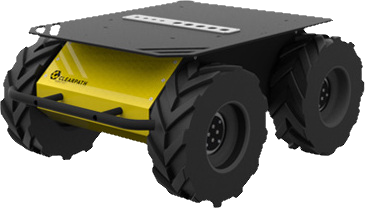
\includegraphics[width = 0.8\textwidth]{Figures/huskyA200.png}
        \caption{Clearpath Husky A200. Image adapted from \cite{clearpath_husky_website}}
        \label{fig:huskyA200}
  \end{minipage}
  \hfill
  \begin{minipage}[b]{0.49\textwidth}
    \centering
    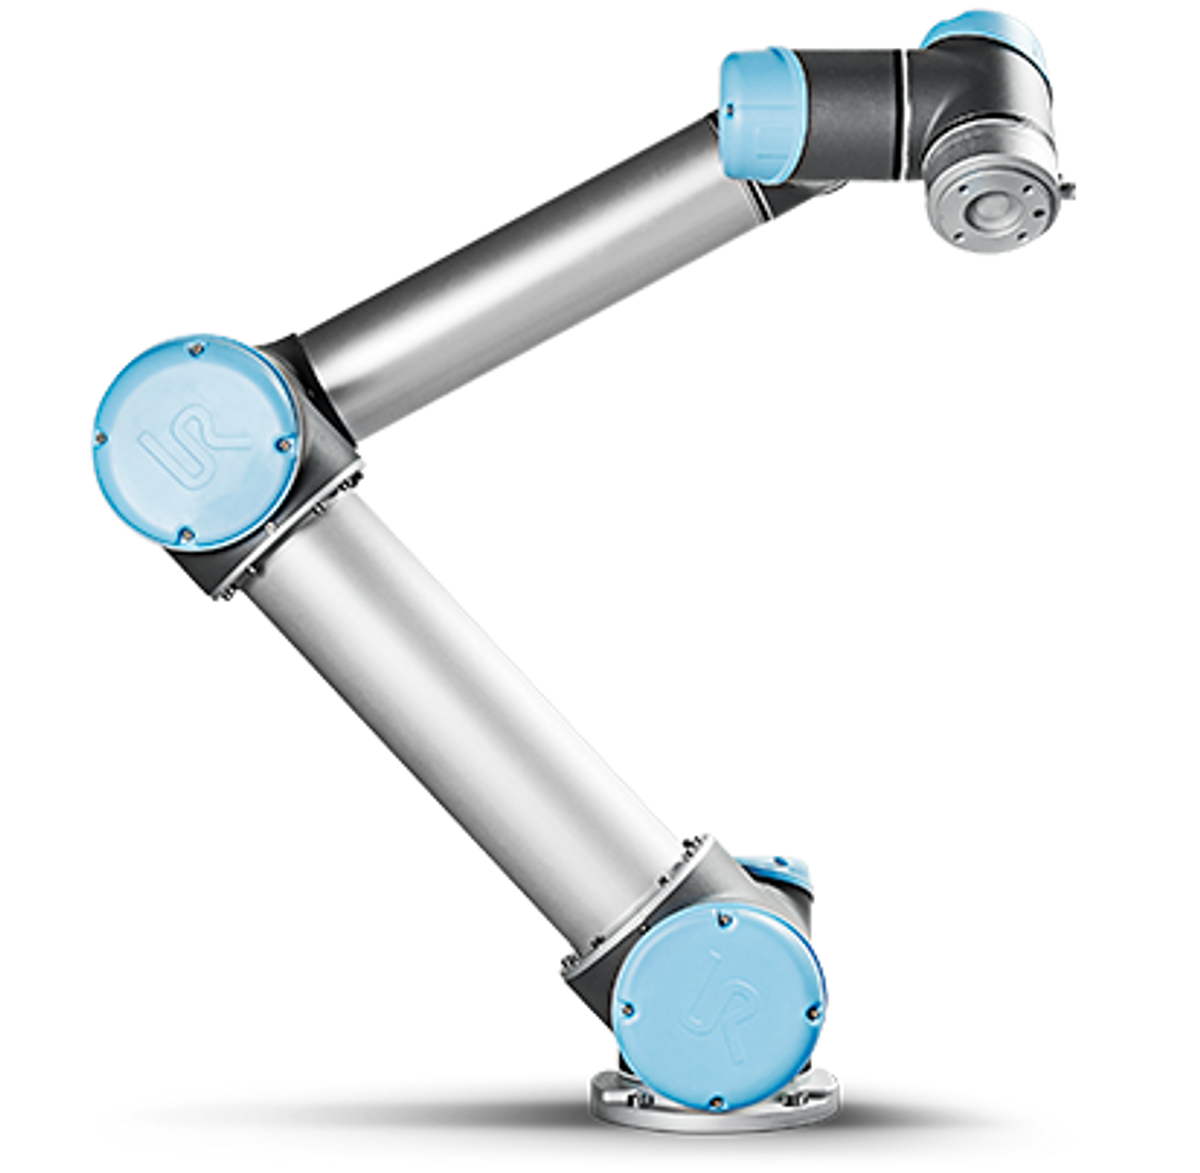
\includegraphics[width = 0.8\textwidth]{Figures/ur5.png}
    \caption{Universal Robots UR5. Image from \cite{ur5_img}}
    \label{fig:ur5}
  \end{minipage}
\end{figure}

Some specifications on the Husky A200 robotic platform is listed in table \ref{tab:husky:a200:specs}

\begin{table}[H]
\centering
\caption{Technical specifications for the Clearpath Husky A200, complete data sheet available in appendix \ref{A:fig:husky_data_sheet}, from \cite{clearpath_husky_website}}
\label{tab:husky:a200:specs}
\vspace{1mm}
\begin{tabular}{ll}
\hline
\multicolumn{2}{c}{\textbf{Husky A200 Specifications}}                                                            \\ \hline
Drivers and APIs                            & ROS, ROS 2, C++ and Python                                          \\
Wheel encoders                              & Quadrature: 78,000 {[}pulses/m{]}
        \\
Communication                               & RS232@115200 Baud                                                   \\
Battery                                     & \begin{tabular}[c]{@{}l@{}}12V 20Ah\\ Sealed Lead Acid\end{tabular} \\
\multicolumn{1}{c}{User Power Distribution} & \begin{tabular}[c]{@{}l@{}}5V 5A\\  12V 5A\\  24V 5A\end{tabular}   \\
Weight                                      & 50 {[}kg{]}                                                         \\
Payload Capacity                            & 75 {[}kg{]}                                                         \\
External Dimensions                         & 990 x 670 x 390 {[}mm{]}                                            \\ \hline
\end{tabular}
\end{table}

One NVIDIA Jetson AGX Xavier, hereby called "UGV Xavier", interfaces with Husky, LiDAR and IMU. This computer will control the Husky and take care of autonomous navigation tasks such as mapping, localization and path planning. 

The second NVIDIA Jetson AGX Xavier, hereby called Manipulator Xavier, interfaces with the Realsense camera and robotic manipulator. This computer will control the manipulator, and take care of sensory information from the Realsense camera. 

The relatively powerful GPU of the Xaviers adds capabilities to implement deep learning algorithms to do for example image- or PointCloud based object detection.

\subsection{Final Design/Concept??}

The UR5 manipulator requires a dedicated controller to operate.This controller also contains the DC-power supply for the manipulator. As the manipulator is to be mounted on an UGV, this controller has to be powered through DC-power. According to the Universal Robots CB3 battery supply installation manual \cite{ur5_battery_manual}, the UR5 could draw up to 50A at "peak conditions". Looking at table \ref{tab:husky:a200:specs}, it is clear that the built in 24V power distribution on the Husky, with a 5A circuit breaker, is insufficient.

\begin{figure}[H]
  \centering
  \begin{minipage}[b]{0.49\textwidth}
        \centering
        The design of a mobile power system for the CB3 controller and thus, the UR5 manipulator is beyond the scope of this project. The decision was therefore made to swap out the UR5 manipulator with a smaller Interbotix VX300 manipulator from Trossen Robotics, illustrated in figure \ref{fig:vx300}. This is a significantly smaller robotic arm that is powered through 12V DC-power supply with a standard 2.5mm DC barrel jack. 
  \end{minipage}
  \hfill
  \begin{minipage}[b]{0.49\textwidth}
   \centering
  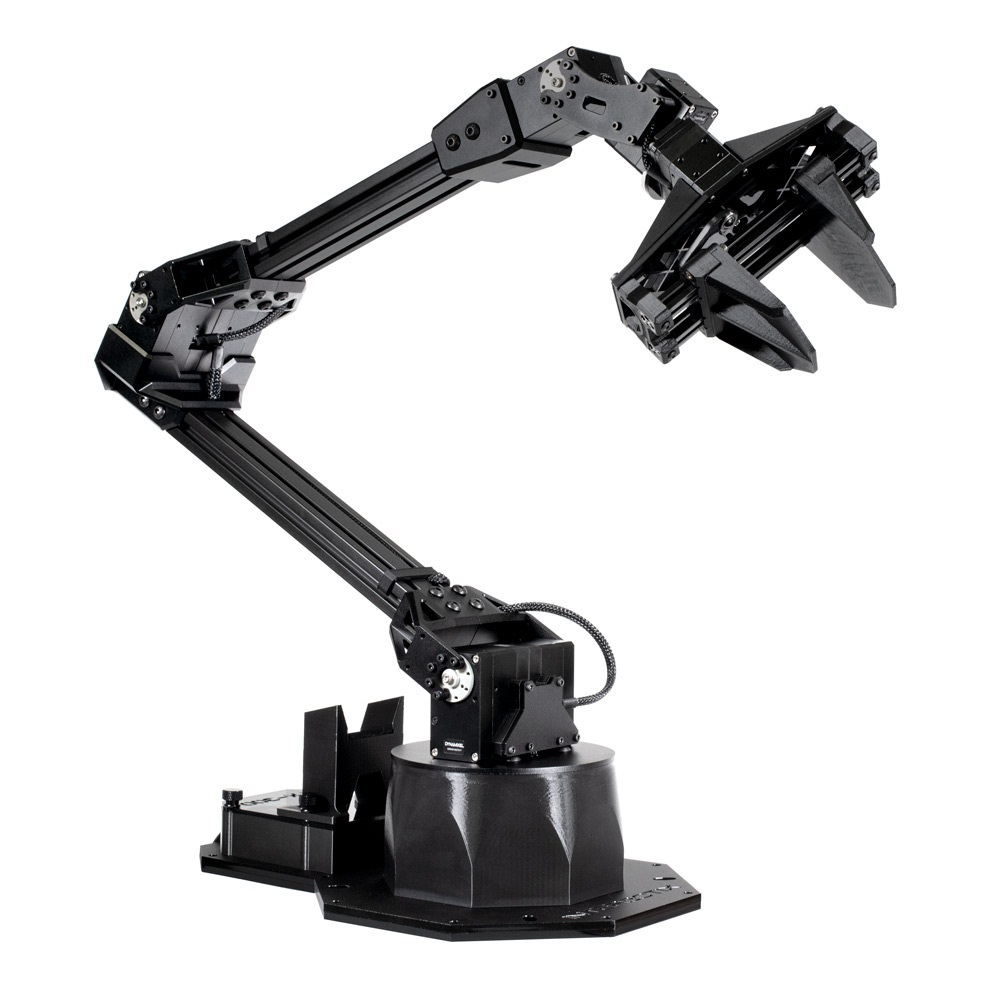
\includegraphics[width = 0.7\textwidth]{Figures/VX300.jpg}
  \caption{Interbotix Vx300. Image from \cite{interbotix_vx300}}
  \label{fig:vx300}
  \end{minipage}
\end{figure}
  
\section{Hardware}
This section describes the different hardware components of the robotic system and how they are set up for this project. A high level overview of the network topology is shown in figure \ref{fig:topology}. This topology gives an insight to how the different components are connected to create a complete system. Looking at figure \ref{fig:topology}, it can be seen that the UGV Xavier communicates with the Husky through RS232 and the UM7 IMU through USB. The LiDAR communicates through Ethernet via a WiFi router that, in this case acts as a switch. The LiDAR data is therefore available for all computers on the network. From figure \ref{fig:topology}, it can be seen that the Manipulator Xavier interfaces with both the Realsense camera and the manipulator through USB. 

\begin{figure}[H]
  \centering
  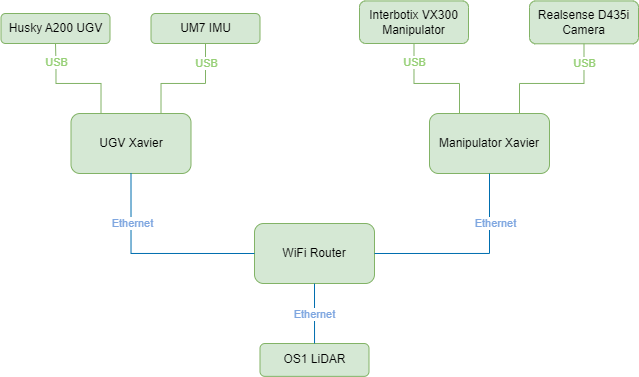
\includegraphics[width = 0.6\textwidth]{Figures/example_figure.drawio.png}
  \caption{High level network topology showing the various components on the mobile robotic platform}
  \label{fig:topology}
\end{figure}

The WiFi Router allows external computers to connect to the network, either through WiFi or cabled connection, and communicate with the two Xaviers and the LiDAR. This makes it possible to control the Xavier computers through SSH and also allows developers to interact with the ROS2 network.

\subsection{General Arrangement}
The UGV acts as a bracket that holds all sensors and actuators as well as having the role of powering all equipment it holds. A general arrangement drawing describing physical arrangement of all the components mounted on the UGV is presented in figure \ref{fig:general_arrangement}.

\begin{figure}[H]
  \centering
   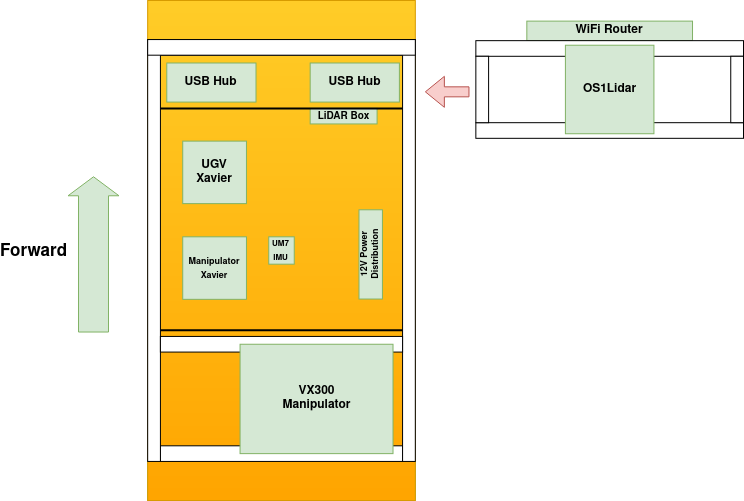
\includegraphics[width = 0.9\textwidth]{Figures/general_arrangement.drawio.png}
  \caption{General arrangement drawing of UGV platform. Here, the physical position of different hardware components are defined. The sensor frame is drawn to the left of the main frame to make it easier to read.}
  \label{fig:general_arrangement}
\end{figure}


\subsection{Electrical Interface}
The different components in the system is powered through the user power supply of the UGV(see table \ref{tab:husky:a200:specs}). Figure \ref{fig:circuit_diagram} is a circuit diagram that illustrates the DC power distribution.

\begin{figure}[H]
  \centering
  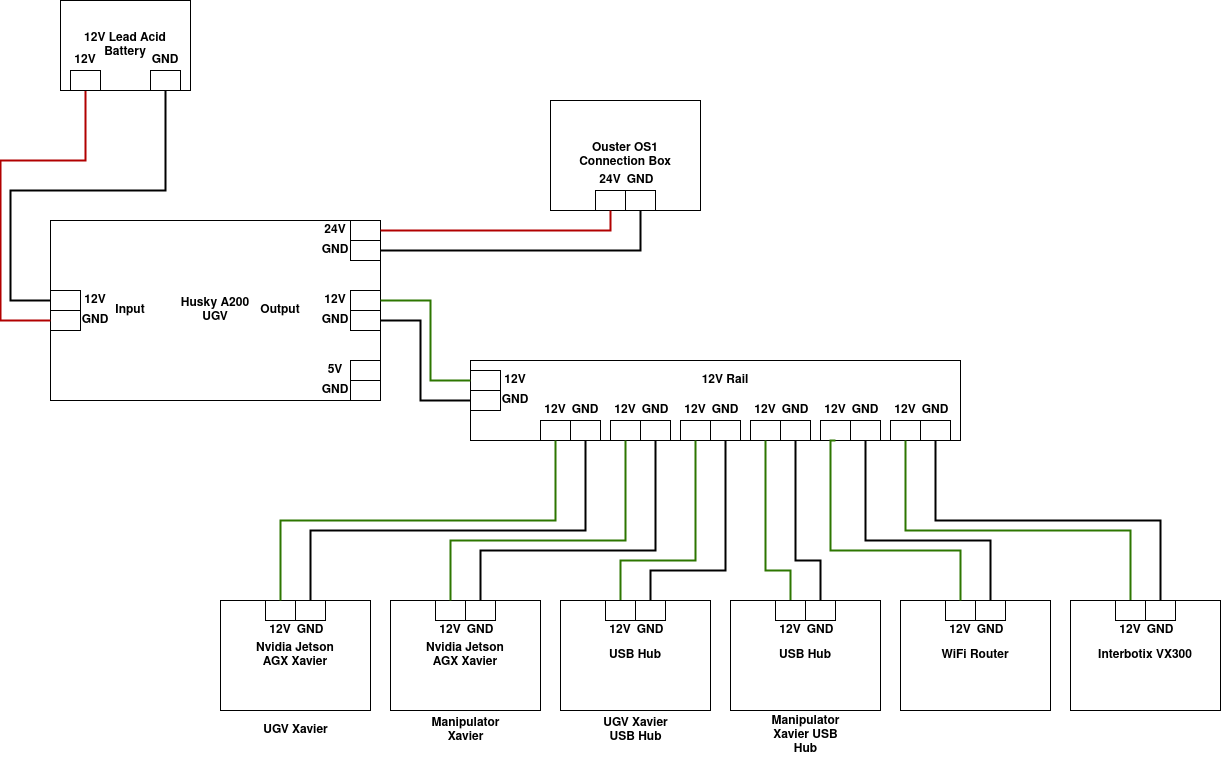
\includegraphics[width = 1\textwidth]{Figures/circuit_diagram.drawio.png}
  \caption{Circuit diagram showing the power distribution on the UGV}
  \label{fig:circuit_diagram}
\end{figure}



\subsubsection{Sensor mounting frame}


The complete setup is described in URDF files, which allows for an accurate digital model of the robot to be made . The URDF model of the robot is shown in figure \ref{fig:hardware}.

\begin{figure}[H]
  \centering
  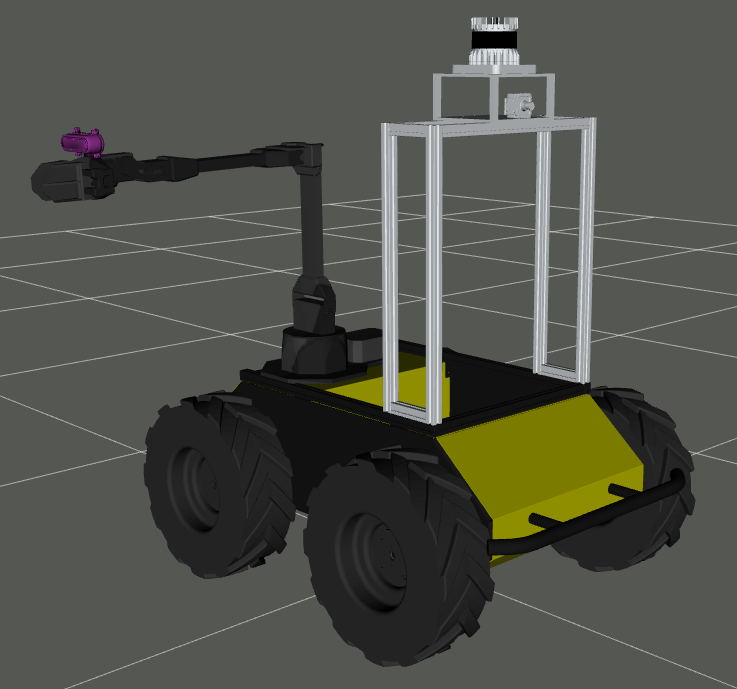
\includegraphics[width = 0.6\textwidth]{Figures/husky_initiated.png}
  \caption{3D model of the robotic system.}
  \label{fig:hardware}
\end{figure}

\subsubsection{IMU}

\subsubsection{LiDAR}

\subsection{Manipulator}

\subsection{Machine Vision Camera}

\section{Software Setup}

\subsection{ROS2 Setup}

\subsection{UGV Setup}
\subsubsection{Model Description}

\subsection{IMU Setup}

\subsection{LiDAR Setup}

\subsection{IMU Fusion}

\subsection{Manipulator}
\subsubsection{Model Description}
\subsubsection{Panning Scene}

\subsection{Machine Vision}
\subsubsection{Camera Setup}
\subsubsection{Apriltag}


\section{Autonomous Navigation}
Autonomous navigation is achieved using the NAV2 navigation stack for ROS 2.

\subsection{SLAM}

\subsection{Navigation 2}



\section{Algorithms}

\subsection{Scene Geometry Publisher}

\subsection{Husky Pick and Place}


\subsection{Husky Master Node}
On a high level, the system is controlled by a ros node called "husky\_master". This node interacts with NAV2 and Moveit 2 to orchestrate an autonomous pick and place operation. The interaction between "husky\_master" and Moveit 2 is done through "husky\_pick\_and\_place" which acts as an interface between Moveit 2 and "husky\_master". A high level overview of this interaction is shown in figure \ref{fig:husky_master}

\begin{figure}[H]
  \centering
  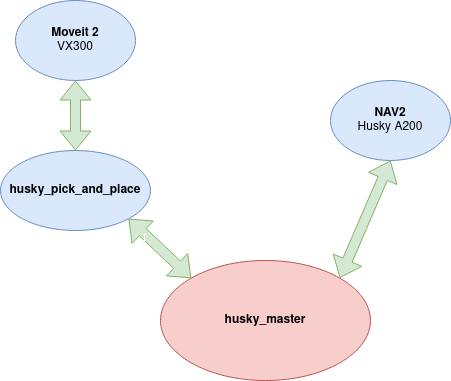
\includegraphics[width = 0.6\textwidth]{Figures/software_overview.drawio.png}
  \caption{The "husky\_master" node controls the operation by interfacing directly with NAV2 and with Moveit2 through the "husky\_pick\_and\_place" node.}
  \label{fig:husky_master}
\end{figure}
